
\item A cylindrical cavity of diameter \( a \) exists inside a cylinder of diameter \( 2a \) as shown in the figure. Both the cylinder and the cavity are infinitely long. A uniform current density \( J \) flows along the length.

If the magnitude of the magnetic field at the point \( P \) is given by \(\frac{N}{12} \mu_0 aJ \), then the value of \( N \) is \underline{\hspace{2.5cm}}.
    \begin{center}
        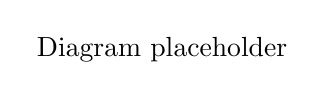
\begin{tikzpicture}
            % Diagram here - as I cannot generate complex figures, please replace this with appropriate TikZ commands.
            \node at (0, 0) {Diagram placeholder};
        \end{tikzpicture}
    \end{center}
